\documentclass[a4paper,12pt]{article}
\usepackage{pgfplots}
\usepackage{tikz}
\usepackage{custom} % contains goldfish colors
\usepackage[margin=1in,footskip=0.25in]{geometry}
\usepackage{subcaption}
\usepgfplotslibrary{fillbetween}
\usetikzlibrary{fadings}
\tikzfading[name=myfading]
\pgfplotsset{compat=1.15}
\usetikzlibrary{plotmarks}


\usepgfplotslibrary{external}
\tikzexternalize[prefix=tikz_figures/]

\begin{document}
\begin{figure}[h]  

\begin{tikzpicture}

\begin{semilogxaxis}[	
	axis on top,
	enlargelimits=true,
	scale only axis,
	height=0.3\textwidth,
   	width=0.4\textwidth,
	xlabel={ $Ra$}, ylabel={ $\sigma$},
	xlabel style={yshift=0.08cm,xshift=.cm},
	ylabel style={xshift=-0.0cm,yshift=-0.0cm},
	%xtick pos=left,
	%ytick pos=left,
	every tick/.style={black},
	major tick length=.1cm,
	minor tick length=.5mm,
	xmin=1.2e3,
	xmax=2.e4,
	xtick={1e3,1e4,1e5},
	clip=false,
	%xticklabels={16,32,64,128},
	%legend style = {font=\footnotesize},
	%legend style={nodes={scale=0.8}},
	%legend pos = south east,
   ] 


% Single Roll
\addplot[draw=c6,fill=black!90, solid,mark=square*, only marks,mark size=2.3]
 table[x expr=\thisrowno{0},y expr=\thisrowno{1}] {../zero_onset.txt};
 %\addlegendentry{1-roll}
 
% Double Roll
\addplot[draw=black,fill=gfred3, solid,mark=*, only marks,mark size=2.7]
 table[x expr=\thisrowno{0},y expr=\thisrowno{2}] {../zero_onset.txt};
 %\addlegendentry{2-roll (h)}
 
% Double Roll
\addplot[draw=black,fill=gfblue3, solid,mark=diamond*, only marks,mark size=3.5]
 table[x expr=\thisrowno{0},y expr=\thisrowno{3}] {../zero_onset.txt};
 %\addlegendentry{2-roll (v)}
 
% Double Roll
\addplot[draw=black,fill=yelc1, solid,mark=triangle*, only marks,mark size=3.5]
 table[x expr=\thisrowno{0},y expr=\thisrowno{4}] {../zero_onset.txt};
 %\addlegendentry{4-roll}\\
 
\draw[dashed] ({rel axis cs:0,0}|-{axis cs:0,0}) -- ({rel axis cs:1,0}|-{axis cs:0,0});

% -- Images
\node [above right,inner sep=0pt,clip=false] at (8.7e2,.55) (a) {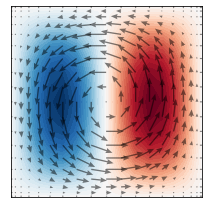
\includegraphics[width=1.6cm]{../single.png}};
\node [right,inner sep=0pt,clip=false] at (a.east) (b) {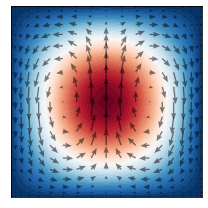
\includegraphics[width=1.6cm]{../doublh.png}};
\node [right,inner sep=0pt,clip=false] at (b.east) (c) {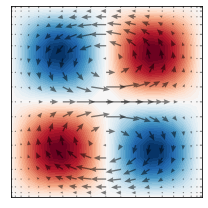
\includegraphics[width=1.6cm]{../doublv.png}};
\node [right,inner sep=0pt,clip=false] at (c.east) (d) {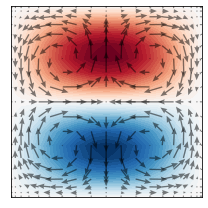
\includegraphics[width=1.6cm]{../quadru.png}};
\node [above, color=black] at (a.north) {1-roll};
\node [above, color=gfred3] at (b.north) {2-roll$^h$};
\node [above, color=gfblue3] at (c.north) {2-roll$^v$};
\node [above, color=yelc1] at (d.north) {4-roll};
%\draw[-latex,inner sep=0pt,gray] (a) -- (0.1,1.4e6);

% \addplot[color=black,opacity=0.7,no markers,dashed]
% coordinates { (3e11, 0.026)(3e11, 0.107)};

%\addlegendentry{ejecting (GF)}

\path[name path=A] (rel axis cs:0,1) -- (rel axis cs:1,1);
\path[name path=B] (rel axis cs:0,0.78) -- (rel axis cs:1,0.78);
\tikzfillbetween[of=A and B]{gray, opacity=0.2};
\node [above, color=black] at (rel axis cs:0.85,0.02) {stable};
\node [above, color=black] at (rel axis cs:0.2,0.8) {unstable};
\end{semilogxaxis}
%\node[ align=center, text=black] at (-1.4,5.2) {a)}; 
\end{tikzpicture}% NO EMPTY LINE HERE!!!! 

\end{figure}  

\end{document}